\documentclass{standalone}
\usepackage{tikz}

\begin{document}

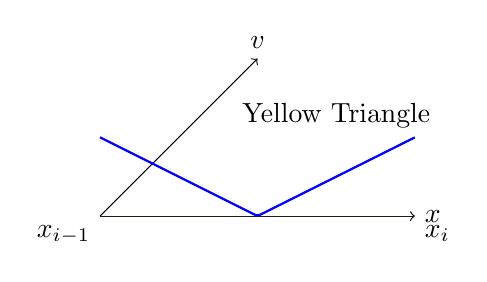
\begin{tikzpicture}[scale=2]

% Define coordinates
\coordinate (x0) at (-1, 0);
\coordinate (x1) at (1, 0);
\coordinate (y1) at (0, 1);

% Draw the x-axis
\draw[->] (x0) -- (x1) node[right] {$x$};

% Draw the y-axis
\draw[->] (x0) -- (y1) node[above] {$v$};

% Fill the yellow triangle
\fill[yellow!50] (x0) rectangle (x1) |- cycle;

% Add labels
\node at (x0) [below left] {$x_{i-1}$};
\node at (x1) [below right] {$x_i$};
\node at (0.5, 0.5) [above] {Yellow Triangle};

% Draw the function v(x)
\draw[blue, thick] plot[domain=-1:1, samples=100] (\x, {0.5 * abs(\x)});

\end{tikzpicture}

\end{document}